%!TEX root = JUrban_SOFT2014.tex

\section{Results} % (fold)
\label{sec:results}

We have selected five time slices from COMPAS shots 4275 and 6962 (i.e. 10 cases in total) for the analysis. These cases include circular, elongated and diverted plasmas with different currents. 

\subsection{Example cases}

A comparison of plasma shapes for shot 4275 is shown in Fig. \ref{fig:ex4275}. Numerical values of reconstruction errors are presented in Table \ref{table:ex4275}. We can observe a very good agreement between the original equilibrium and the reconstructed shapes. In this case, FREEBIE was using linear $p'$ and $FF'$ polynomials so that the EFIT++ model agrees with the target data. VacTH uses 8 magnetic probes and 16 flux loops. As we discuss later, flux loops are essential for reliable VacTH results. Even global kinetic properties are well reconstructed in EFIT++; the largest error around 10~\% is in $l_{\mathrm i}$ (i.e. basically in the toroidal current density profile).

\begin{table*}
\centering
\small
\begin{tabular}{lrrrrrrrrrrrrr}
\toprule
   code &  time &  $\left| \Delta R_{\mathrm in} \right|$ &  $\left| \Delta R_{\mathrm out} \right|$ &  $\left| \Delta Z_{\mathrm min} \right|$ &  $\left| \Delta Z_{\mathrm max} \right|$ &  $\delta \kappa$ &  $E_\mathrm{mp}$ &  $E_\mathrm{fl}$ &  $\delta W$ &  $\delta l_{\mathrm i}$ &  $\delta \beta_{\mathrm p}$ &  $\delta q_0$ &  $\delta q_{95}$ \\
\midrule
 EFIT++ &  0.97 &              0 &            0.002 &        0.001 &        0.001 &                  0.003 &       0.001 &      0.0009 &          0.04 &           0.09 &              0.03 &           0.03 &           0.007 \\
 EFIT++ &  0.99 &          4e-05 &            9e-05 &        0.001 &        0.001 &                  0.004 &       0.001 &      0.0006 &          0.04 &           0.09 &              0.04 &           0.02 &           0.005 \\
 EFIT++ &  1.02 &         0.0005 &           0.0002 &        0.002 &        0.002 &                  0.008 &       0.002 &       0.002 &          0.02 &            0.1 &              0.02 &           0.02 &           0.009 \\
 EFIT++ &  1.05 &          0.001 &           0.0008 &        4e-05 &       0.0003 &                  0.004 &       0.003 &       0.005 &          0.01 &           0.07 &              0.02 &           0.01 &           0.009 \\
 EFIT++ &   1.1 &          0.001 &           0.0005 &        0.005 &       0.0002 &                  0.005 &       0.004 &       0.002 &          0.04 &           0.09 &              0.03 &           0.02 &            0.05 \\
  VacTH &  0.97 &              0 &            0.001 &       0.0006 &       0.0002 &                  0.002 &       8e-07 &       7e-05 &           -- &            -- &               -- &            -- &             -- \\
  VacTH &  0.99 &          4e-05 &           0.0004 &        0.001 &       0.0008 &                  0.004 &       4e-07 &      0.0001 &           -- &            -- &               -- &            -- &             -- \\
  VacTH &  1.02 &          0.002 &           0.0008 &        0.005 &        0.002 &                   0.01 &       2e-06 &       0.002 &           -- &            -- &               -- &            -- &             -- \\
  VacTH &  1.05 &          0.006 &            0.002 &        5e-05 &        0.002 &                   0.01 &       3e-06 &        0.02 &           -- &            -- &               -- &            -- &             -- \\
  VacTH &   1.1 &          0.005 &            0.002 &        0.002 &        0.003 &                   0.02 &       2e-06 &       0.003 &           -- &            -- &               -- &            -- &             -- \\
\bottomrule
\end{tabular}

\caption{Errors for the same cases as in Fig. \ref{fig:ex4275}.}
\label{table:ex4275}
\end{table*}

\begin{figure*}
\centering   %\begin{center}
\hfill{}
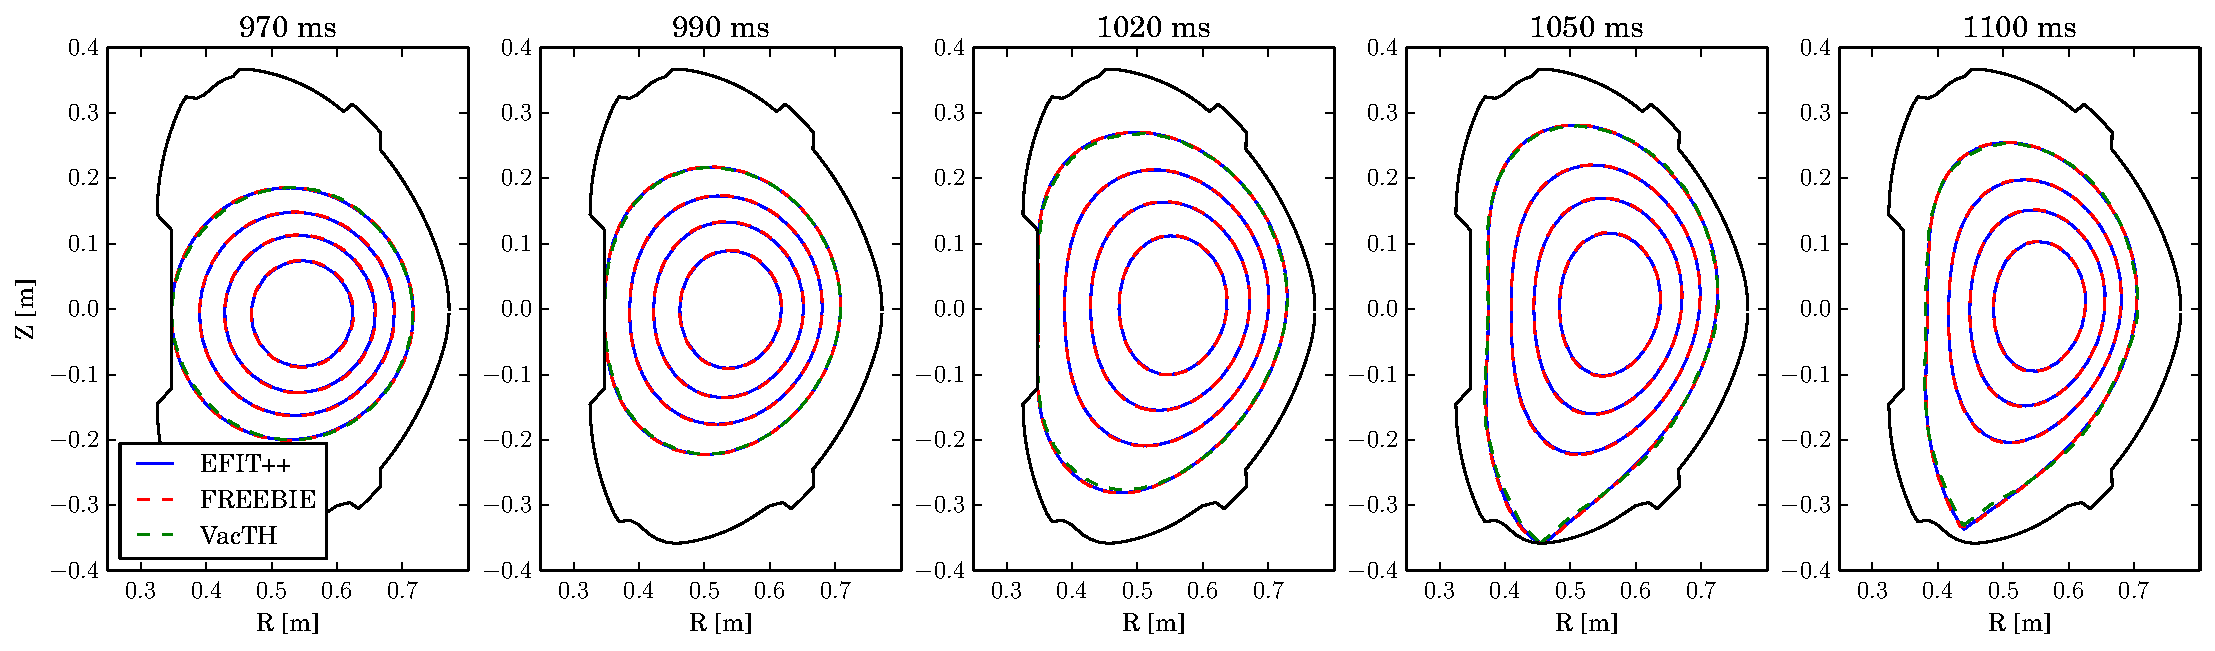
\includegraphics[width=18cm]{figures/example_4275.pdf}
\hfill{}
%\end{center}
\caption{Contours of $\bar\psi=\left(0.25,0.5,0.75,1\right)$, reconstruction from FREEBIE data, shot 4275. EFIT++ parameters: $n_\mathrm{mp} = 16$, $n_\mathrm{fl} = 4$, $n_{p'} = n_{FF'} = 1$. VacTH parameters: $n_\mathrm{mp} = 8$, $n_\mathrm{fl} = 16$, $n_P = n_Q = 5$. $E_\mathrm{mp, fl}$ is the relative error of the reconstructed magnetic probes and flux loops values, respectively.}
\label{fig:ex4275}
\end{figure*}


The second shot for the comparison is 6962, which has been chosen because Thomson scattering (TS) profiles are available. In Fig. \ref{fig:ex6962} we show reconstructions for more realistic equilibria and an artificial noise in the synthetic diagnostic signals. TS pressures were used in FREEBIE equilibria, which course no longer feature linear $p'$ and $FF'$ profiles. 
It is apparent that the reconstruction is not as good as in the previous case. Nevertheless, the plasma shape is well reconstructed with EFIT++ and VacTH, except for the last time slice in which VacTH yields too large plasma in the upper part.
$n_P = n_Q = 4$ is used in this case as these values are minimum for reasonable VacTH results, while higher values are too sensitive to the input noise.
Expectedly, EFIT++ reconstruction with magnetic data only cannot reliably reconstruct kinetic plasma parameters, such as the stored energy or $q_0$. Rather unexpected is a relatively good agreement of $l_\mathrm{i}$. However, this agreement is compensated by a large error of $\beta_{\mathrm p}$ so that the quantity $\beta_{\mathrm p} + l_{\mathrm i}/2$ remain within a 10~\% error bar. Notable are large errors (up to 40~\%) in the stored energy, which are mainly caused by incompatible pressure profiles.

\begin{figure*}
\centering   %\begin{center}
\hfill{}
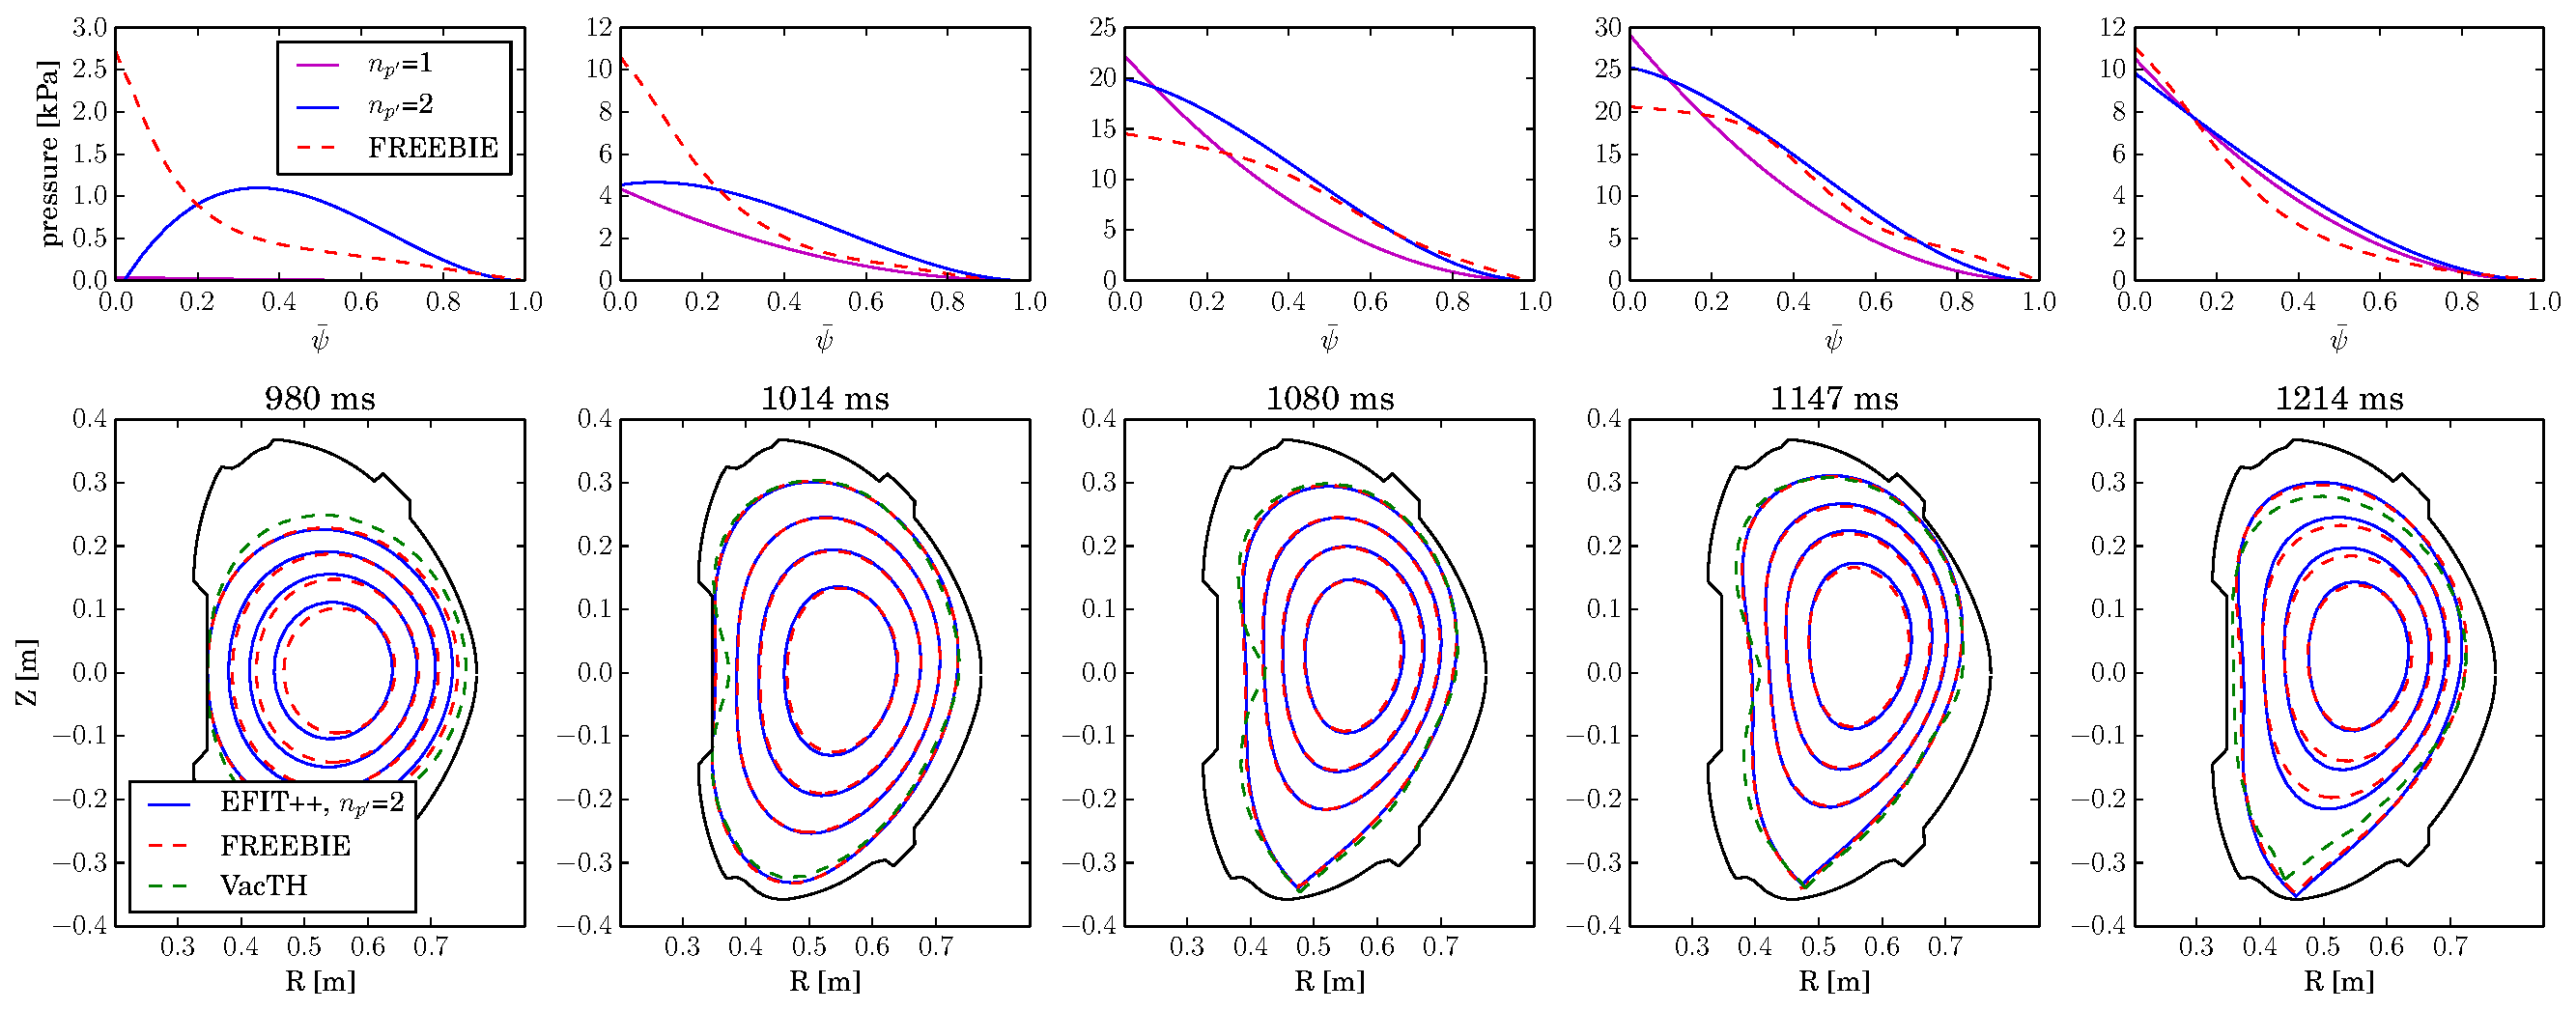
\includegraphics[width=18cm]{figures/example_6962_TS_noise.pdf}
\hfill{}
%\end{center}
\caption{Pressure profiles and contours of $\bar\psi=\left(0.25,0.5,0.75,1\right)$, reconstruction from FREEBIE data with 3~\% random noise, shot 6962 with Thomson scattering pressure profiles. EFIT++ parameters: $n_\mathrm{mp} = 16$, $n_\mathrm{fl} = 4$, $n_{FF'} = 1$. VacTH parameters: $n_\mathrm{mp} = 8$, $n_\mathrm{fl} = 16$, $n_P = n_Q = 4$.}
\label{fig:ex6962}
\end{figure*}

\begin{table*}
\centering
\small
\begin{tabular}{lrrrrrrrrrrrrr}
\toprule
   % code &  time &  $\Delta R_{\mathrm in}$ &  $\Delta R_{\mathrm out}$ &  $\Delta Z_{\mathrm min}$ &  $\Delta Z_{\mathrm max}$ &  $\delta \kappa$ &  $E_\mathrm{mp}$ &  $E_\mathrm{fl}$ &  $\delta W$ &  $\delta \left(\beta_{\mathrm p} + l_{\mathrm i}/2 \right)$  &  $\delta q_0$ &  $\delta q_{95}$ \\
   code &  time &  $\left| \Delta R_{\mathrm in} \right|$ &  $\left| \Delta R_{\mathrm out} \right|$ &  $\left| \Delta Z_{\mathrm min} \right|$ &  $\left| \Delta Z_{\mathrm max} \right|$ &  $\delta \kappa$ &  $E_\mathrm{mp}$ &  $E_\mathrm{fl}$ &  $\delta W$ &  $\delta l_{\mathrm i}$ &  $\delta \beta_{\mathrm p}$ &  $\delta q_0$ &  $\delta q_{95}$ \\
\midrule
 EFIT++ &    980 &               0 &            0.009 &       -0.003 &        0.003 &                   0.01 &        0.04 &        0.01 &           0.1 &            0.3 &               0.1 &            0.5 &            0.02 \\
 EFIT++ &   1014 &          0.0004 &          -0.0005 &       -0.001 &        0.001 &                  0.002 &        0.01 &        0.01 &         0.006 &            0.1 &             0.003 &           0.07 &           0.003 \\
 EFIT++ &   1080 &          -0.002 &           -0.002 &       -0.002 &        0.002 &                  0.003 &        0.01 &        0.02 &           0.2 &            0.1 &               0.2 &           0.06 &            0.02 \\
 EFIT++ &   1147 &          -0.002 &          -0.0006 &       -0.007 &       -0.002 &                  0.006 &        0.01 &        0.02 &           0.1 &            0.2 &               0.1 &            0.2 &            0.01 \\
 EFIT++ &   1214 &          -0.004 &            0.007 &        0.006 &       -0.004 &                   0.04 &        0.03 &        0.01 &           0.2 &            0.3 &               0.2 &           0.03 &           0.001 \\
  VacTH &    980 &               0 &            -0.01 &         0.01 &        -0.02 &                   0.04 &      0.0002 &        0.01 &           -- &            -- &               -- &            -- &             -- \\
  VacTH &   1014 &           0.006 &           -0.003 &        -0.01 &       -0.001 &                   0.02 &       7e-05 &        0.02 &           -- &            -- &               -- &            -- &             -- \\
  VacTH &   1080 &            0.01 &           -0.003 &        0.004 &       -0.003 &                   0.01 &       3e-05 &       0.009 &           -- &            -- &               -- &            -- &             -- \\
  VacTH &   1147 &            0.02 &           -0.003 &       -0.002 &        0.002 &                   0.04 &       5e-05 &        0.01 &           -- &            -- &               -- &            -- &             -- \\
  VacTH &   1214 &            0.01 &            0.001 &        -0.02 &         0.02 &                   0.07 &      0.0001 &        0.01 &           -- &            -- &               -- &            -- &             -- \\
\bottomrule
\end{tabular}
\caption{Errors for the same cases as in Fig. \ref{fig:ex6962}.}
\label{table:ex6962}
\end{table*}


\begin{figure*}
\centering   %\begin{center}
\hfill{}
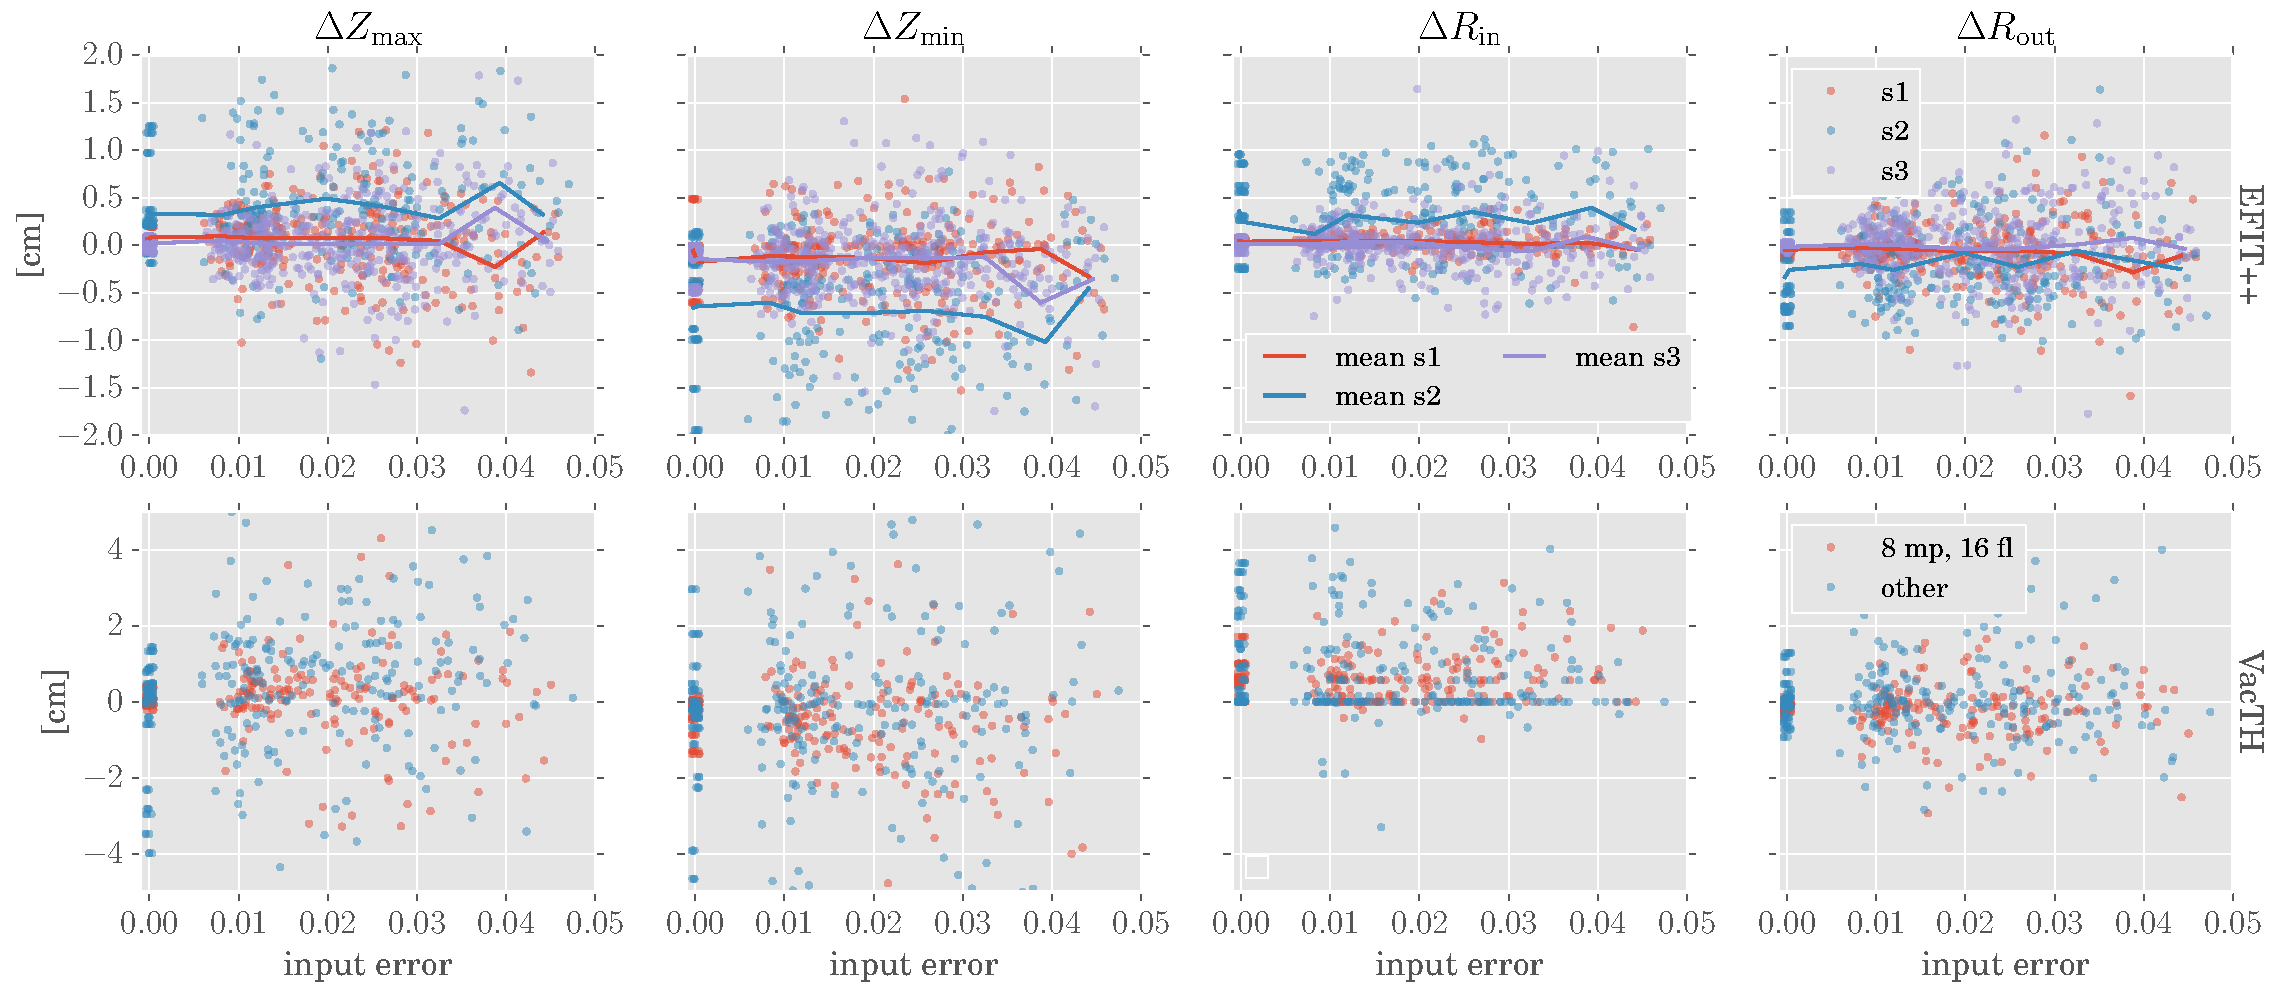
\includegraphics[width=18cm]{figures/RZstats.pdf}
\hfill{}
%\end{center}
\caption{Absolute errors in LCFS extents for convergent cases. EFIT++ results in the first row, VacTH in the second row. S1 denotes linear $p'$ and $FF'$ in EFIT++ as well as FREEBIE, s2 denotes TS pressure profiles in FREEBIE and $n_{p'} = n_{FF'} = 1$ in EFIT++, s3 denotes TS pressure profiles in FREEBIE and $n_{p'} = 2$ in EFIT++. Full lines show the means. VacTH parameters are $n_P=n_Q=4$, ``8 mp, 16 fl'' denotes $n_\mathrm{mp}=8$, $n_\mathrm{fl}=16$. Input error is calculated as an average of $I_{\rm{p}}$, magnetic probes and flux loops values. Zero input error data are scattered for a better visibility.}
\label{fig:RZstats}
\end{figure*}

\begin{figure*}
\centering   %\begin{center}
\hfill{}
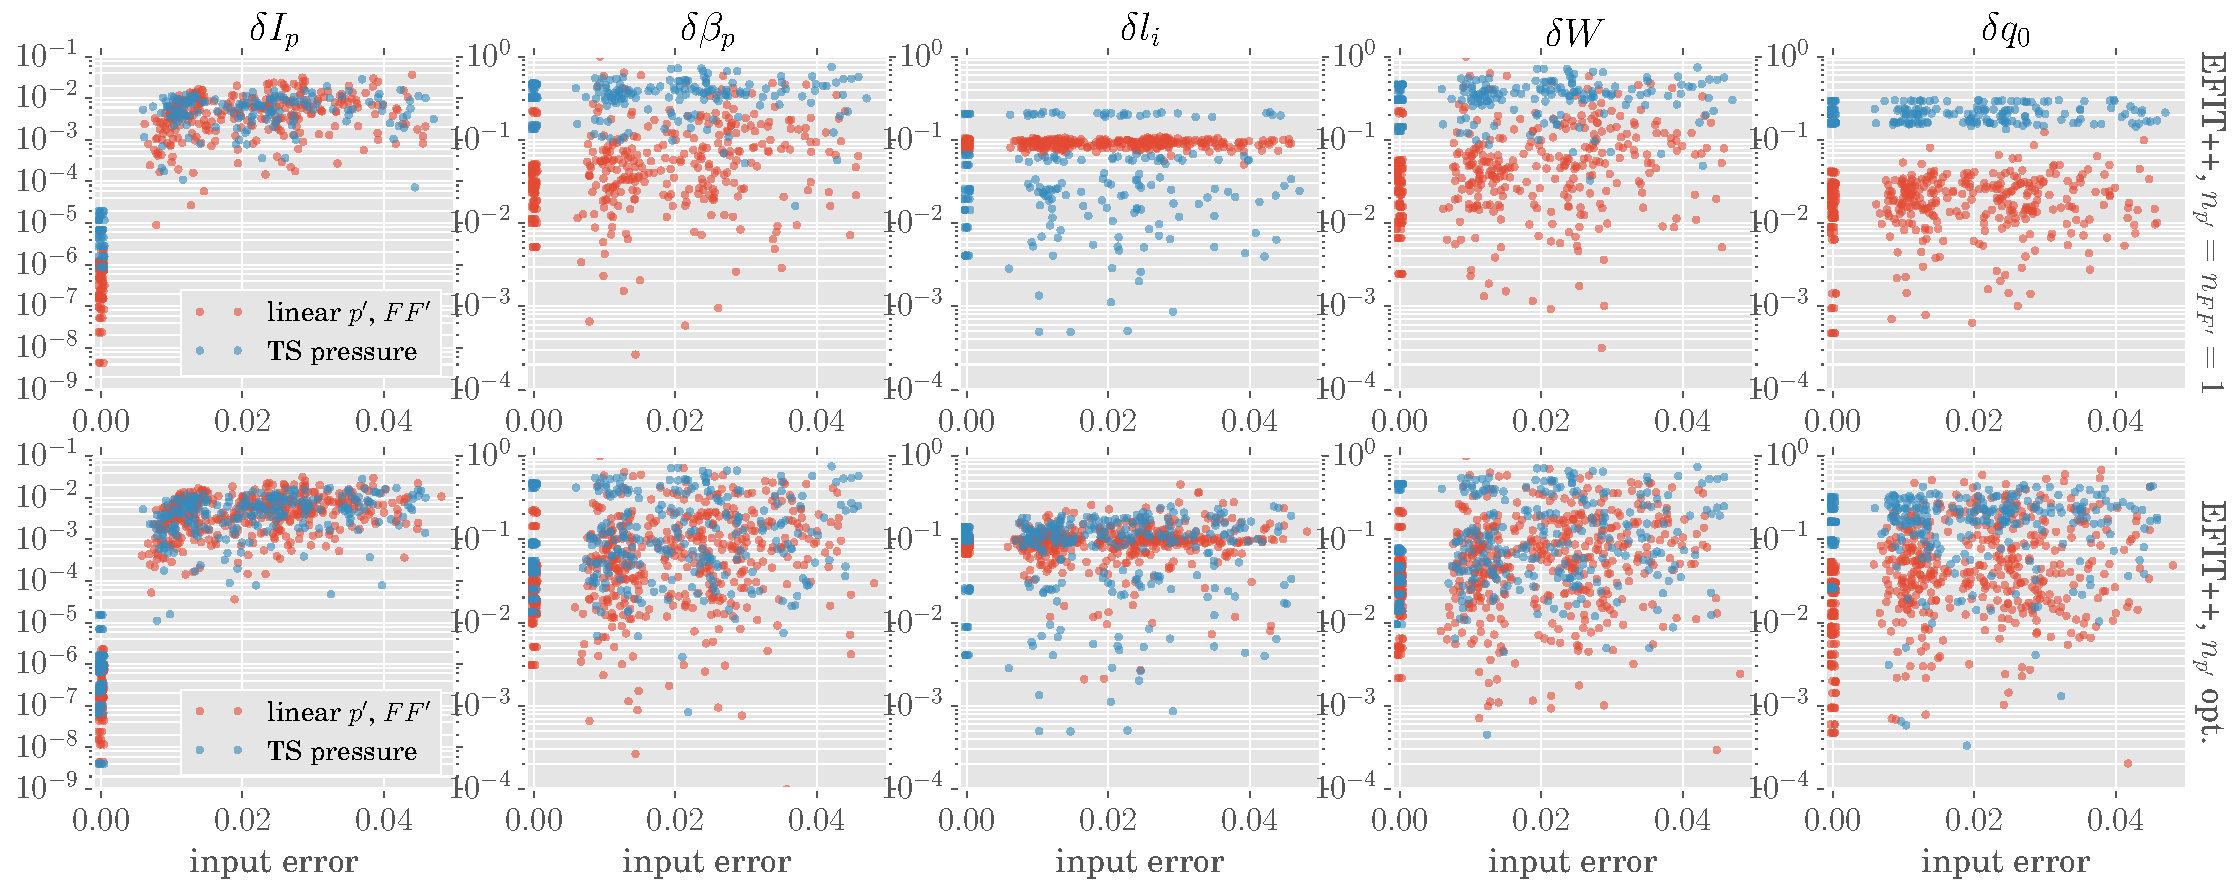
\includegraphics[width=18cm]{figures/kinetic_stats_opt.pdf}
\hfill{}
%\end{center}
\caption{Internal plasma parameters relative errors for EFIT++ reconstructions using $n_{p'}=n_{FF'}=1$ in the top row and more optimized $n_{p'}$ in the bottom row. Zero input error data are scattered for a better visibility.}
\label{fig:kinetic_stats}
\end{figure*}


\subsection{Statistical analysis} % (fold)
\label{sub:statistical_analysis}

In order to get a global overview of EFIT++ and VacTH reconstruction properties on COMPASS, we perform a scan over major code parameters and signal noise levels. In particular, $n_{p',FF'} = 1,2 $, $(n_\mathrm{mp}, n_\mathrm{fl}) = (16, 4), (64, 4), (8, 16)$, $\epsilon = 0, 0.02, 0.04, 0.06$, $n_{P,Q} = 4, 5, 6$. The same cases as above (time slices of shots 4275 and 6962) are used as target equilibria. For shot 6962, equilibria with TS pressure profiles and with linear $p'$ and $FF'$. This means there is 15 different target equilibria in total.

Absolute errors of the reconstructed LCFS extents for convergent cases from the scan are shown in Fig. \ref{fig:RZstats}. We can observer that the LCFS reconstructed with EFIT++ for target linear $p'$ and $FF'$ profiles (selection 1) are within 1~cm errors. There are, however, cases with up to 3 cm errors in $Z_{\rm{min}}$ for the more realistic TS pressure profiles (selection 2) if $n_{p'}=1$ is used. This error can be reduced by using $n_{p'}=2$. Input errors do not pose major difficulties for EFIT++. 

VacTH is performing reasonably well for its most favourable diagnostic set of 8 magnetic probes and 16 flux loops and $n_P = n_Q = 4$. With a higher number of harmonics or with less flux loops, VacTH becomes unreliable and yields significant errors. Unfortunately, only 4 flux loops are currently available on COMPASS. In fact, it is easier for VacTH to fit magnetic probes than flux loops while magnetic probes do not fully determine the magnetic flux. This is also apparent in $E_\mathrm{mp}$ and $E_\mathrm{fl}$ values in Tables \ref{table:ex4275} and \ref{table:ex6962}. An additional optimization of the fitting weights or algorithm is probably needed. The current behaviour might be quite anti-intuitive as VacTH performs significantly worse with 16 flux loops and 16 or 64 magnetic probes in comparison to 16 flux loops and only 8 magnetic probes. 

EFIT++ internal plasma parameters reconstruction results are shown in Fig. \ref{fig:kinetic_stats}. It shows that purely magnetic reconstruction with $n_{p'}=n_{FF'}=1$ introduces (except for $I_{\rm{p}}$) a systematic error for realistic pressure profiles, i.e. for plasmas that do not have the same profile parametrization. 
It is known that magnetic reconstruction with EFIT is difficult for limited plasmas (without additional constraints, particularly the store energy) \cite{efit1985}.
This suggests that using $n_{p'}=1$ for limited plasmas and $n_{p'}=2$ for diverted plasmas might lead to better results. This is demonstrated in the bottom row of Fig. \ref{fig:kinetic_stats}.
Reconstructions with such optimized parameters do not suffer from the systematic error; however, they generally increase the error bars for target equilibria with linear $p'$ and $FF'$, especially for $q_0$. It is also notable that $\delta l_{\rm{i}} \cong 0.1$ for all $n_{p'}=n_{FF'}=1$ reconstructions.

\begin{figure}
\centering   %\begin{center}
\hfill{}
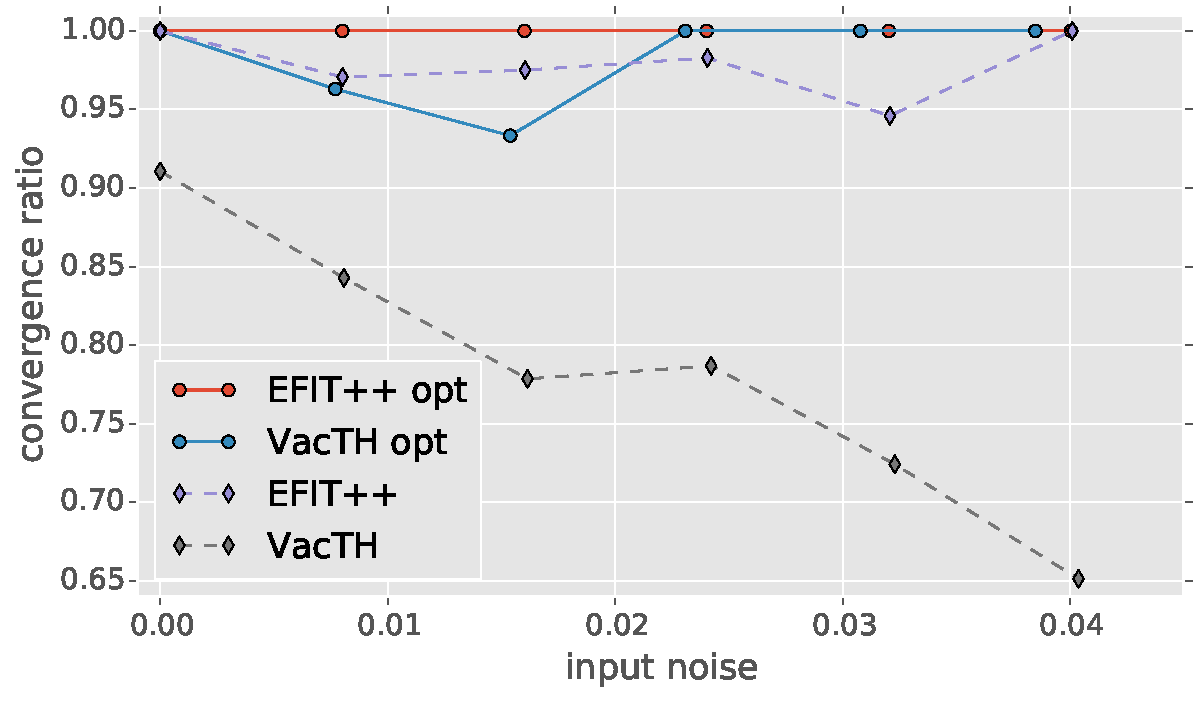
\includegraphics[width=8cm]{figures/convergence_ratio_6962.pdf}
\hfill{}
%\end{center}
\caption{Ratio of converged cases to all cases, shot 6962, TS profiles. Opt refers to optimized code parameters.}
\label{fig:convergence_ratio}
\end{figure}

Another important property is the converged cases ratio, shown in Fig. \ref{fig:convergence_ratio}. EFIT++ converges in almost all cases with any of the tested configurations and in 100~\% cases in the optimized configuration (i.e. with $n_{p'}=2$ for diverted plasmas). $n_P = n_Q = 4$ must be used in VacTH unless the number of non-converged cases is too large. 
Quite interestingly, optimized VacTH convergence rate drops significantly around 2~\% input noise.

% subsection statistical_analysis (end)


% section results (end)
